\section{Imágenes Dataset} \label{anexo:dataset}

\begin{figure}
    \centering
    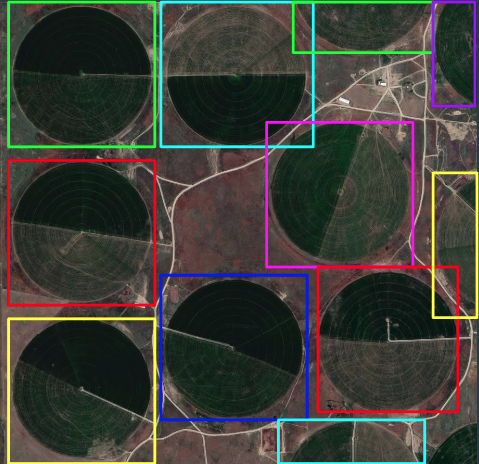
\includegraphics[width=0.9\textwidth]{img/pivot etiquetado manual - 1.png}
    \caption{Pívot etiquetado manualmente}
    \label{Pivot etiquetado manualmento 1}
\end{figure}

\begin{figure}
    \centering
    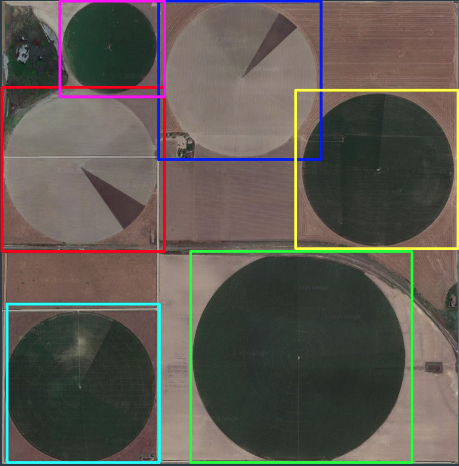
\includegraphics[width=0.9\textwidth]{img/pivot etiquetado manual - 2.png}
    \caption{Pívot etiquetado manualmente}
    \label{Pivot etiquetado manualmento 2}
\end{figure}

\begin{figure}
    \centering
    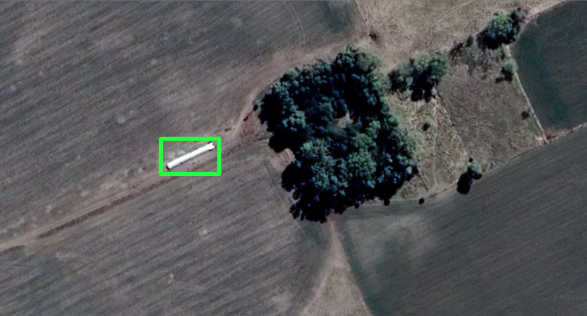
\includegraphics[width=0.9\textwidth]{img/silobolsa etiquetado manual - 1.png}
    \caption{Silobolsa etiquetado manualmente}
    \label{Silobolsa etiquetado manualmento 1}
\end{figure}

\begin{figure}
    \centering
    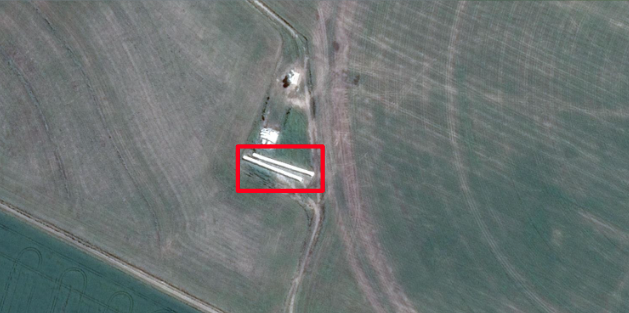
\includegraphics[width=0.9\textwidth]{img/silobolsa etiquetado manual - 2.png}
    \caption{Silobolsa etiquetado manualmente}
    \label{Silobolsa etiquetado manualmento 2}
\end{figure}

\begin{figure}
    \centering
    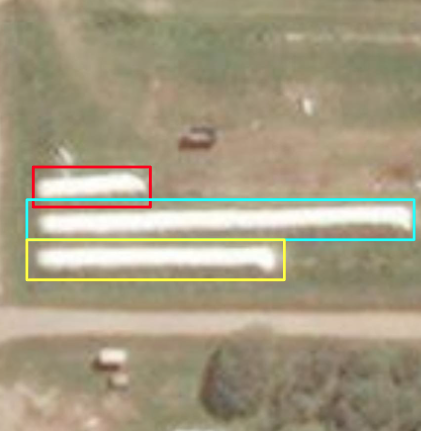
\includegraphics[width=0.9\textwidth]{img/silobolsa etiquetado manual - 3.png}
    \caption{Silobolsa etiquetado manualmente}
    \label{Silobolsa etiquetado manualmento 3}
\end{figure}

\begin{figure}
    \centering
    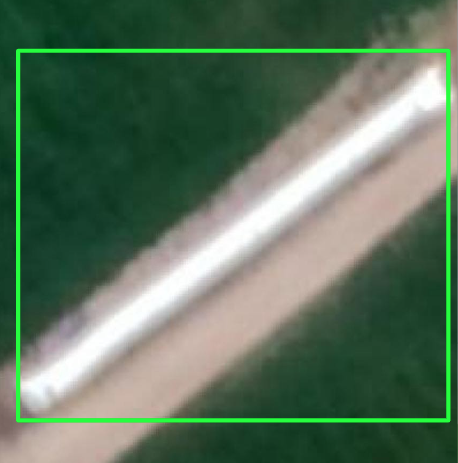
\includegraphics[width=0.9\textwidth]{img/silobolsa etiquetado manual - 4.png}
    \caption{Silobolsa etiquetado manualmente}
    \label{Silobolsa etiquetado manualmento 4}
\end{figure}

\begin{figure}
    \centering
    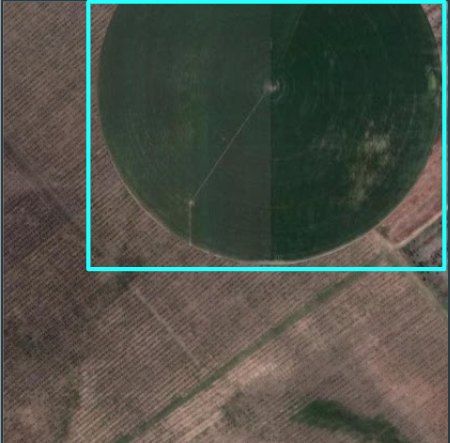
\includegraphics[width=0.9\textwidth]{img/pivot data aug - 1.png}
    \caption{Pívot generado con data augmentation}
    \label{Pivot generado con data augmentation 1}
\end{figure}

\begin{figure}
    \centering
    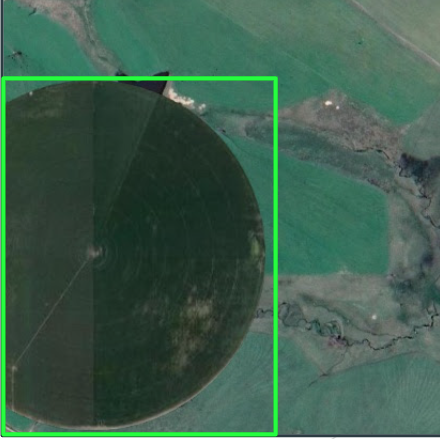
\includegraphics[width=0.9\textwidth]{img/pivot data aug - 2.png}
    \caption{Pívot generado con data augmentation}
    \label{Pivot generado con data augmentation 2}
\end{figure}

\begin{figure}
    \centering
    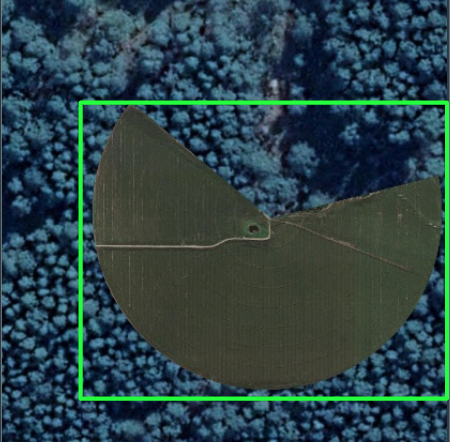
\includegraphics[width=0.9\textwidth]{img/pivot data aug - 3.png}
    \caption{Pívot generado con data augmentation}
    \label{Pivot generado con data augmentation 3}
\end{figure}

\begin{figure}
    \centering
    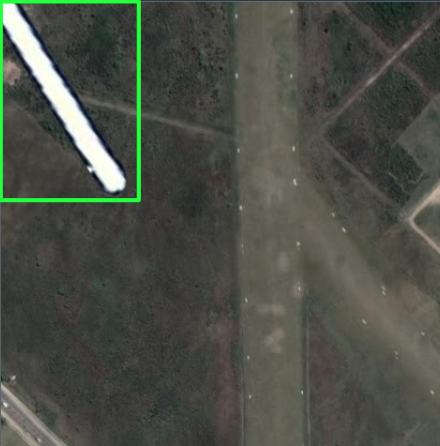
\includegraphics[width=0.9\textwidth]{img/silobolsa data aug - 1.png}
    \caption{Silobolsa generado con data augmentation}
    \label{Silobolsa generado con data augmentation 1}
\end{figure}

\begin{figure}
    \centering
    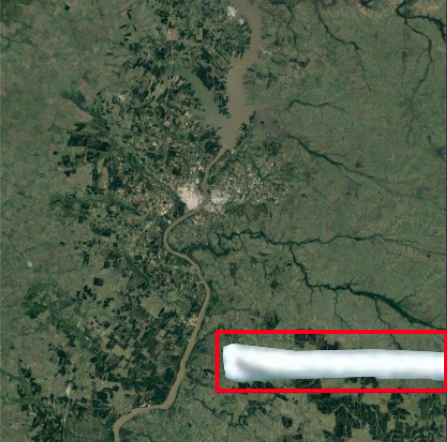
\includegraphics[width=0.9\textwidth]{img/silobolsa data aug - 2.png}
    \caption{Silobolsa generado con data augmentation}
    \label{Silobolsa generado con data augmentation 2}
\end{figure}
